\begin{frame}
    \frametitle{Topological Spaces}
    The following questions deal with the idea of Topological Spaces, so here's a quick recap on what exactly those are.\\\\
    \textbf{Topological Spaces:} A \textit{topological space} is a set $X$ on which a \textit{topology} $\tau$ is equipped. $\tau$ is a collection of subsets of $X$ (or, $\tau$ is a subset of the power set $2^{X}$ of $X$) such that -

    \begin{enumerate}
        \item $\varnothing$ and $X$ should belong to $\tau$
        \item the union of the elements in any subset of $\tau$ should belong to $\tau$
        \item the intersection of the elements in any finite subset of $\tau$ should belong to $\tau$
    \end{enumerate}
\end{frame}

\begin{frame}
    The elements of $\tau$ are called \textit{open sets}. Thus, a topological space is a pair $(X, \tau)$ consisting of a set and a topology on it.\\\\
    We can reframe the axioms given on the previous slide in terms of open sets - 
    \begin{enumerate}
        \item The empty and the full set are open.
        \item Any arbitrary union of open sets is open.
        \item Any finite intersection of open sets is open.
    \end{enumerate}
\end{frame}

\begin{frame}
    \frametitle{Problem Set 3.4 - 8}
    \textbf{Show that: The euclidean, diamond, square metrics on $\mathbb{R}^2$ have the same underlying topology. (When we say continuous map from $\mathbb{R}^2$ to $\mathbb{R}$, it is w.r.t this topology.) Further, check that it coincides with the product topology on $\mathbb{R} \times \mathbb{R}$.}\\\\
    Before we jump into the proof for this, which is slightly convoluted, we need to talk about how to compare topologies. The set of all topologies on a set forms a partially ordered set with the binary relation $\subseteq$. With this relation, we can define a partial ordering that we use to compare topologies. \\\\
    If there are two topologies $\tau$ and $\tau'$ on $X$ such that $\tau \subseteq \tau'$, then $\tau$ is said to be a \textit{coarser or weaker topology} than $\tau'$ and $\tau'$ is a \textit{finer or stronger topology} than $\tau$. An additional check is whether the two topologies are equal, if they aren't equal, then one can be called \textbf{strictly} finer or coarser than the other.
\end{frame}

\begin{frame}
    The three metrics in question were defined in the earlier slides, but for the sake of context, the diamond metric $d_1$, the euclidean metric $d_2$ and the square metric $d_\infty$ are defined over $\mathbb{R}^2$ as follows - (note that the notation used is $\boldsymbol{x} = (x_1, x_2)$, $\boldsymbol{y} = (y_1, y_2)$ are points in $\mathbb{R}^2$)
    \begin{gather*}
        d_1(\boldsymbol{x}, \boldsymbol{y}) = |x_1 - y_1| + |x_2 - y_2| \\
        d_2(\boldsymbol{x}, \boldsymbol{y}) = \sqrt{|x_1 - y_1|^2 + |x_2 - y_2|^2} \\
        d_\infty(\boldsymbol{x}, \boldsymbol{y}) = \text{max} \{|x_1 - y_1|, |x_2 - y_2|\}
    \end{gather*}
\end{frame}

\begin{frame}
    Now, let us examine the relation between these three metrics.
    \begin{equation*}
        d_\infty(\boldsymbol{x}, \boldsymbol{y}) = \text{max} \{|x_1 - y_1|, |x_2 - y_2|\} = \left(\text{max} \{|x_1 - y_1|, |x_2 - y_2|\}^2 \right)^{\frac{1}{2}}
    \end{equation*}
    We can also straightaway see that -
    \begin{equation*}
        \text{max} \{|x_1 - y_1|, |x_2 - y_2|\}^2 \leq |x_1 - y_1|^2 + |x_2 - y_2|^2
    \end{equation*}
    Note the fact that $f(x) = x^{\frac{1}{2}}$ is an increasing function for $x \geq 0$. Thus, we have -
    \begin{gather*}
        \left(\text{max} \{|x_1 - y_1|, |x_2 - y_2|\}^2 \right)^{\frac{1}{2}} \leq \sqrt{|x_1 - y_1|^2 + |x_2 - y_2|^2} \\
        \implies d_\infty(\boldsymbol{x}, \boldsymbol{y}) \leq d_2(\boldsymbol{x}, \boldsymbol{y})
    \end{gather*} 
\end{frame}

\begin{frame}
    Now,
    \begin{gather*}
        d_1(\boldsymbol{x}, \boldsymbol{y}) = |x_1 - y_1| + |x_2 - y_2| = \sqrt{\left(|x_1 - y_1| + |x_2 - y_2|\right)^2} \\
        = \sqrt{\left(|x_1 - y_1|^2 + |x_2 - y_2|^2 + 2*|x_1 - y_1|*|x_2 - y_2|\right)} \geq \sqrt{|x_1 - y_1|^2 + |x_2 - y_2|^2} \\
        \implies d_1(\boldsymbol{x}, \boldsymbol{y}) \geq d_2(\boldsymbol{x}, \boldsymbol{y})
    \end{gather*}
    (since \( f(x) = \sqrt{x} \) is an increasing function, and \( 2*|x_1 - y_1|*|x_2 - y_2| \geq 0 \) \\\\
    And since \(d_\infty(\boldsymbol{x}, \boldsymbol{y}) \leq d_2(\boldsymbol{x}, \boldsymbol{y})\), we have the following ordering -
    \begin{equation*}
        d_\infty(\boldsymbol{x}, \boldsymbol{y}) \leq d_2(\boldsymbol{x}, \boldsymbol{y}) \leq d_1(\boldsymbol{x}, \boldsymbol{y})
    \end{equation*}
\end{frame}

\begin{frame}
    Now, consider the following - 
    \begin{gather*}
        d_\infty(\boldsymbol{x}, \boldsymbol{y}) = \text{max} \{|x_1 - y_1|, |x_2 - y_2|\} \geq |x_1 - y_1| \\
        \text{Also, } \text{max} \{|x_1 - y_1|, |x_2 - y_2|\} \geq |x_2 - y_2| \\
        \implies 2*\text{max} \{|x_1 - y_1|, |x_2 - y_2|\} \geq |x_1 - y_1| + |x_2 - y_2| \\
        \implies 2*d_\infty(\boldsymbol{x}, \boldsymbol{y}) \geq d_1(\boldsymbol{x}, \boldsymbol{y})
    \end{gather*}
    Which implies, we have the following ordering -
    \begin{equation*}
        d_\infty(\boldsymbol{x}, \boldsymbol{y}) \leq d_2(\boldsymbol{x}, \boldsymbol{y}) \leq d_1(\boldsymbol{x}, \boldsymbol{y}) \leq 2*d_\infty(\boldsymbol{x}, \boldsymbol{y})
    \end{equation*}
\end{frame}

\begin{frame}
    Now, we have 4 metrics \( d_\infty(\boldsymbol{x}, \boldsymbol{y}), d_2(\boldsymbol{x}, \boldsymbol{y}), d_1(\boldsymbol{x}, \boldsymbol{y}) \text{ and } 2*d_\infty(\boldsymbol{x}, \boldsymbol{y})\). (it is a trivial check to see that $2*d_\infty(\boldsymbol{x}, \boldsymbol{y})$ also forms a metric). Before looking at the notion of open sets mathematically, we take a visual look at what open balls of the same radius look like, w.r.t each of these metrics. \\
    \begin{center}
        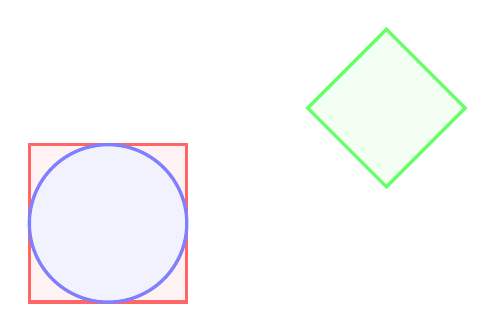
\begin{tikzpicture}
            \filldraw[color=red!60, fill=red!5, very thick](-1,-6) rectangle (1,-4);
            \filldraw[color=blue!50, fill=blue!5, very thick](0,-5) circle (1);
            \filldraw[color=green!60, fill=green!5, very thick, rotate=45](-0.7071, -5.7071) rectangle (0.7071,-4.2929);
        \end{tikzpicture}
    \end{center}
\end{frame}